\chapter{CryptDB as a Software}
\label{chp:software}

Although CryptDB is mainly a proof of concept rather than a commercial software, the source code is available along with instructions on how to install it. This chapter will cover the installation and setup of CryptDB's proxy server, how to connect the proxy server to a regular database system, and finally a small demo application will be presented.

\section{Installation of CryptDB's Software}

CryptDB comes as a software available through MIT, and can be downloaded using the version control system Git. As the creators has moved on to other projects, the source code has not been maintained since 2014, and is currently only tested on Ubuntu 12.04 and Ubuntu 13.04. During the installation of CryptDB, some issues has been encountered. As CryptDB is only tested with said Ubuntu versions, developers are in need of installing the software on such operating systems. This often involves running some sort of \gls{vm} in some \gls{vmm}, which is very inconvenient when developing applications that should be able to run regardless of operating system and environment. When working inside a \gls{vm} with software that is, at best, ready for alpha testing, you better watch your steps. 

\subsection{Docker to the Rescue}

%\begin{wrapfigure}{r}{3cm}
%\centering
%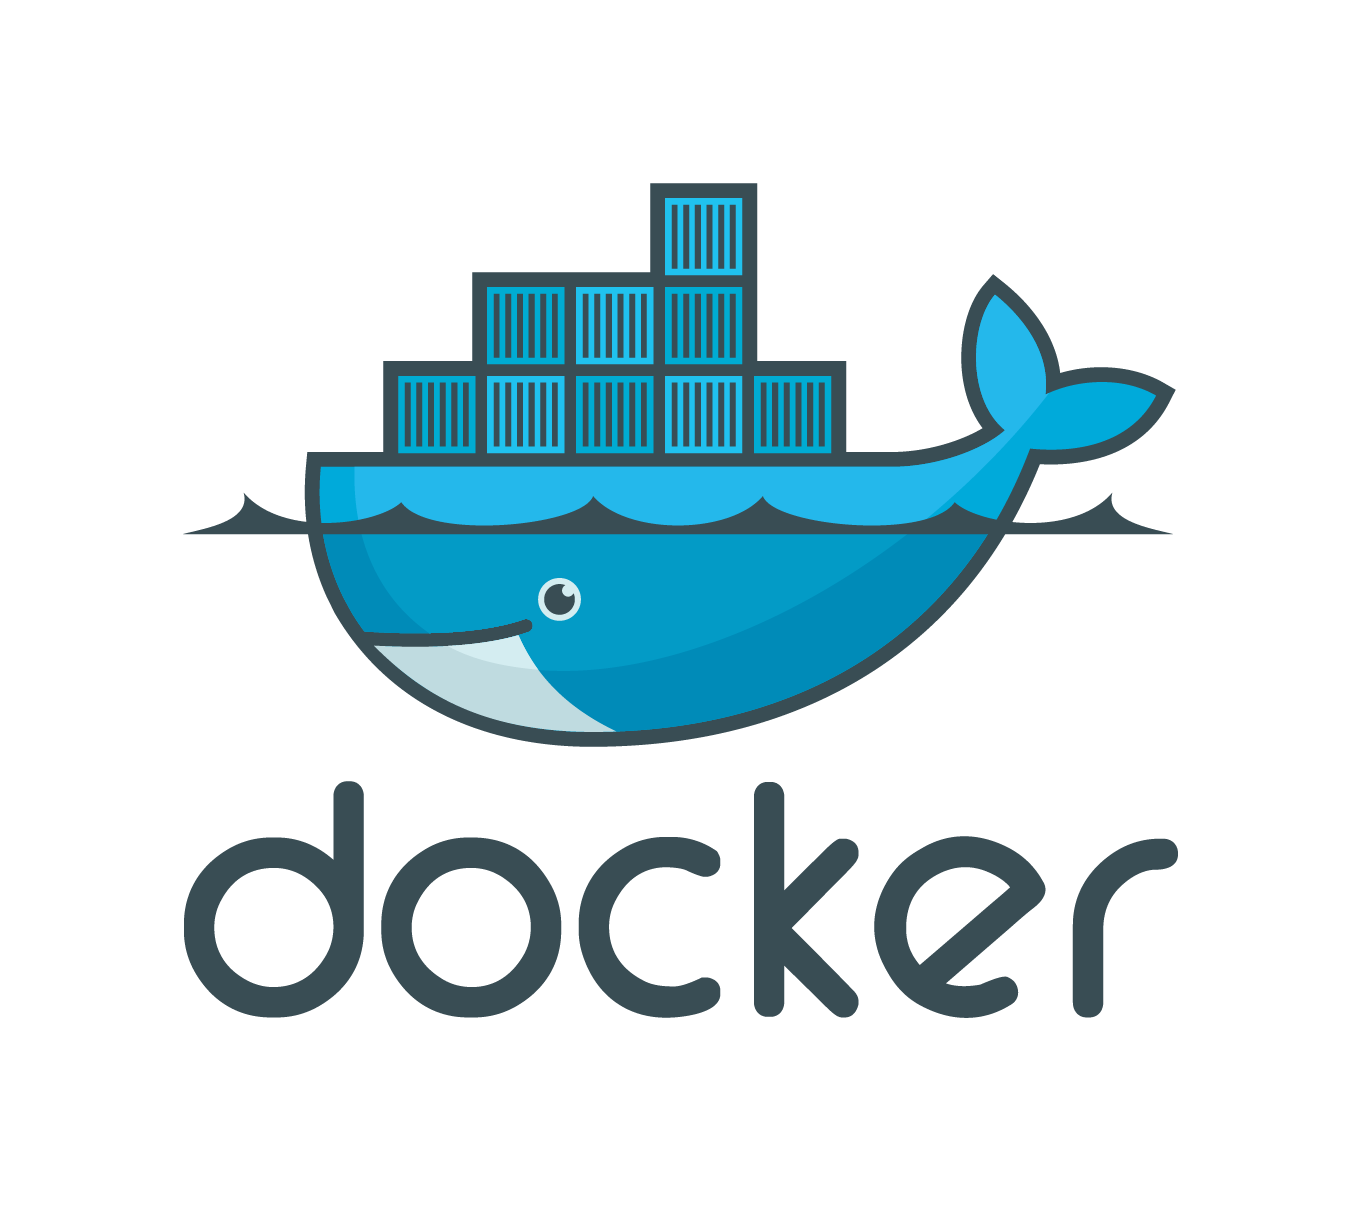
\includegraphics[scale=0.15]{docker.png}
%\caption{Docker}
%\label{fig:docker}
%\end{wrapfigure}
Because of the presented reasons, some of the work related to this project has been to detach CryptDB from such requirements and providing a workable environment regardless of operating system which is easy to reboot if one where to "step on the wrong files". Docker \cite{docker_homepage} is an open-source software allowing programs to be wrapped up in \emph{containers}. Containers are complete file systems containing every piece of code, 
library and dependency the program need to run properly, which runs directly on the host OS without the need of \gls{vmm} and Guest OSs. After a container is built, it can be shipped and run in other environments such as Windows, OS X and Linux without issues.

A thorough guide for installing CryptDB can be found at \url{https://github.com/klevstad/CryptDB_Docker}

\section{A Small Demo Application}

How big should a demo application be? What should be in here?


\section{Discussion of CryptDB as a Software}

Should I compare CryptDB to another HE-database. Perhaps MuteDB ? \url{http://ieeexplore.ieee.org/stamp/stamp.jsp?tp=&arnumber=6977940}




The authors of CryptDB has taken the idea further with Mylar (\url{https://css.csail.mit.edu/mylar/} which I assume to be CryptDB 2.0, or at least building on the main idea. Have not studied yet.